% Crucial Preamble
\documentclass[12pt,letterpaper]{article} \usepackage{amsmath} \usepackage{graphicx} \usepackage[margin=1in]{geometry} \usepackage{longtable}  \usepackage{amssymb}

% Extra Preamble
\usepackage{fancyhdr} \usepackage{enumitem} \usepackage{float} \usepackage{soul}
\usepackage{multicol} \usepackage[compact]{titlesec}


% frames with display breaks
\usepackage{mdframed}
\allowdisplaybreaks

% change spacing
\usepackage{setspace}
\setlength{\parskip}{0.4\baselineskip}

% Remove paragraph indentation
\setlength{\parindent}{0pt}

% Reduce space before and after section headings
%\titlespacing*{\section}{0pt}{0.1\baselineskip}{0.2\baselineskip}

% changes font
%\renewcommand{\familydefault}{\sfdefault}

% adds header and footer
\pagestyle{fancy}
\fancyhead{} \fancyhead[C]{CSI 2110 Cheat Sheet} \fancyhead[L]{CSI2110} \fancyhead[R]{Owen Daigle}
\fancyfoot{} \fancyfoot[C]{\thepage}


\begin{document}
	
	\begin{center}
		\Large\textbf{CSI 2110 Cheat Sheet} \\
		\vspace{0.5em}
	\end{center}
	
	\section{Analysis}
	We analyse algorithmns using the Big Oh notation. 
	
	A big Oh of O(n) means that the worst case running time of the algorithm is n.
	
	We say f(n) is O(g(n)) if there exist positive constants $n_0$ and c such that $f(n)\le cg(n) \forall n\ge n_0$.
	
	\begin{mdframed}
		\textbf{Ex. } Prove the following: 
		
		1. $2n^2 + 10n^3$ is O$(n^3)$
		We need to find the constants c and n0. 
		\begin{align*}
			2n^2 + 10n^3 \le 2n^3 + 10n^3 \le 12n^3 \implies c=12, n_0 = 1
		\end{align*}
		Since the constants exist, then it is proven.
	\end{mdframed}

	Big Omega is similar but it is the best case running time. 
	
	Big theta is the exact time. An algorithm of $\Theta(n)$ ALWAYS takes n time.
	
	\section{Stacks}
	A stack is a first in last out data type.
	
	We can \verb|push()|, \verb|pop()| to add or remove to the top of the stack. There is also \verb|isEmpty()|, \verb|peek()| (returns but does not remove the top) and \verb|size()|.
	
	\section{Queues}
	Queues are first in first out data types. 
	
	Elements are \textit{enqueued} at the read, and \textit{dequeued} from the front. 
	
	This can be inplemented using a \textbf{circular array, or a linkedlist}. 
	
	\section{Deques}
	A double ended queue (Deque) can be inserted at the front or rear of the queue, and can also be removed at the front or end of the queue. 
	
	A\textbf{ doubly linked list} works well for this. 
	
	\section{Lists/Sequence}
	This is a collection of elements in linear order. 
	
	\subsection{Array List}
	An array list can get from any index \verb|get(i)|, set any index \verb|set(i,e)|, add at any index \verb|add(i,e)|, or remove at any index \verb|remove(i)|.
	
	We want to implement the array lists using an\textbf{ extendable array} (double or increment the size when it gets full)
	
	\subsection{Positional List}
	
	A positional list is a list where we can get the previous or next element given a certain element in the list \verb|addBefore(p,e)|, \verb|addAfter(p,e)|. We can also add first or last \verb|addFirst()|, \verb|addLast()|.
	
	We implement positional lists using \textbf{linked lists}. 
	
	\subsection{Sequence}
	
	This provides all operations from the positional list and array list and has bridge methods as well such as \verb|atIndex(i)| (returns position), \verb|indexOf(p)| (returns index).
	
	This can be implemented using arrays or linked lists. 
	
	With \textbf{arrays}, the index based ops will be fast, but the positional ones will be slow. 
	
	With \textbf{linked lists}, the positional ops will be fast, but the index ones will be slow. 
	
	\section{Priority Queues}
	A priority queue is a queue where each element has a priority (key value pair). 
	
	We can \verb|insert(k,v)| in any order, and we can \verb|removeMin()| or just view \verb|min()|.
	
	If we use a \textbf{sorted sequence}, inserting takes O(n), and removing is O(1). 
	
	If we use an\textbf{ unsorted sequence}, inserting takes O(1), and removing is O(n).
	
	\subsection{Heaps}
	A Heap is a \textbf{complete} binary tree that stores a collection of key value pairs. 
	
	We can do either a \textbf{min heap} (min at top), or a \textbf{max heap} (max at top).
	
	With the min heap, the parent of a node is always greater than the children. 
	
	We implement these using a \textbf{priority queue}. 
	
	To remove from a heap, we remove the top element, then take from the bottom. Then we need to \textbf{downheap }until the heap is fixed. (Downheaping means swap with smallest child until child is bigger)
	
	To add on, we add at the first empty spot at the bottom, and then \textbf{upheap}. (Upheaping means swap with parent until parent is smaller).
	
	\subsection{Heap Construction}
	We use bottom up heap construction to build a heap. This takes O(n).
	
	For this, we start at \textbf{bottom right of heap}, then do a downheap on that parent. Then we go to the right and do it again. When that level is done, go up a level starting on the right. We will end up downheaping each element.  

	
	\section{Maps}
	A map stores and retrieves data based on a \textbf{unique key}. We have \verb|get(k)|, \verb|put(k,v)|, \verb|remove(k)|.
	
	A \textbf{sorted map} also has \verb|firstEntry()|, \verb|lastEntry()|.
	
	We can use an \textbf{ordered sequence} where searching takes O(logn), and inserting/removing take O(n).
	
	We can also use a \textit{better} \textbf{BST} (ideally a balanced one such as AVL) where the worst case search is O(n), but best case is O(logn). Inserting and deleting also depend on search so they are the same.
	
	\section{Trees}
	A tree has \textbf{internal nodes }(nodes with at least 1 child) and \textbf{external nodes }or Leafs (node without children).
	
	A tree is called \textit{binary} if each node has at most 2 children.
	
	We can traverse a binary tree using preorder, inorder, or postorder:
	\begin{enumerate}[noitemsep]
		\item Preorder means visit Root, then Left, then Right
		\item Inorder means visit Left, then Root, then Right
		\item Postorder means visit Left, then Right, then Root
	\end{enumerate}

	A binary tree is called \textbf{full} if each internal node has exactly 2 children.
	
	A binary tree of height h is called \textbf{complete} if the tree of height h-1 is perfect, and the rest of the nodes are added starting on the left.
	\begin{center}
		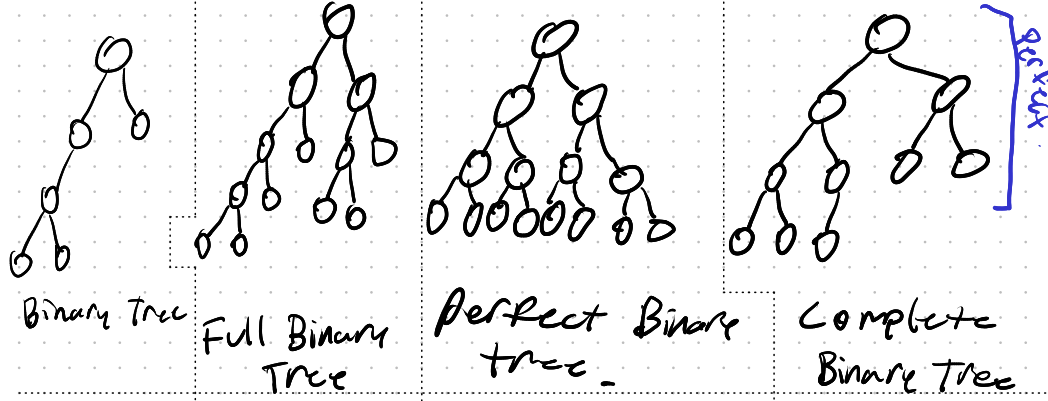
\includegraphics[width=0.8\linewidth]{trees}
	\end{center}

	We have some statistics about a full binary tree: 
	
	n is number of nodes, e is number of external nodes, i is number of internal nodes.
	\begin{align*}
		e = i+1\qquad n=2e-1
	\end{align*}
	These do NOT apply to a general binary tree.
	
	\textbf{All operations (delete, insert) have O(1) except search which depends on the height of the tree}
	
	\subsection{AVL}
	An AVL tree is a BST where each\textbf{ internal node's subtrees heights can differ by at most 1}. This means the \textbf{height is O(logn).}
	
	To insert or delete, we do the same thing as with a BST, except if any change renders the tree unbalanced, we need to rebalance the tree. 
	
	To rebalance, we go to the first node (from the bottom) that is unbalanced, then we do the inorder traversal from it down to the longest side naming the first node visited a, then b, then c. Then we align abc like this with their corresponding subtrees. 
	\begin{center}
		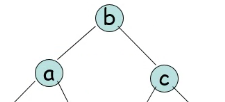
\includegraphics[width=0.2\linewidth]{abdc}
	\end{center}

	\begin{mdframed}[]
	\textbf{Ex. } Remove 7 from this tree.
	\begin{center}
		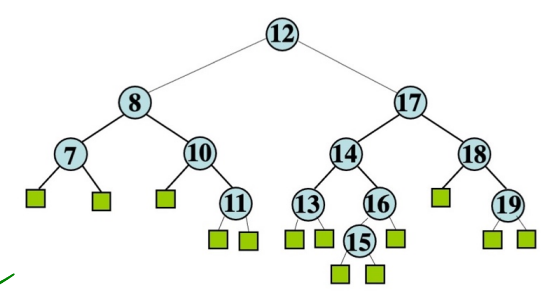
\includegraphics[width=0.4\linewidth]{ex}
	\end{center}
	When removing 7, we see that the 8 is unbalanced. So we do inorder traversal of it and its longest side (10, 11). We assign 8a, 10b, 11c.
	
	So we rearrange like:
	\begin{center}
		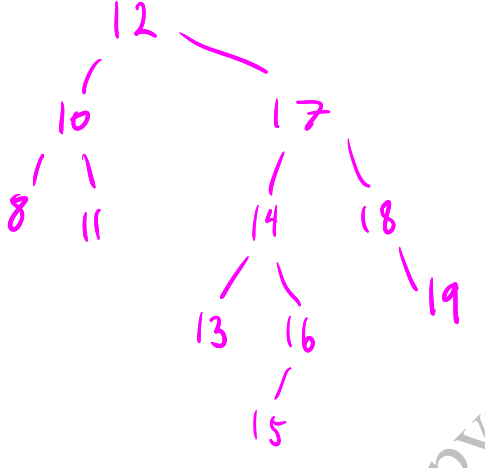
\includegraphics[width=0.3\linewidth]{ex2}
	\end{center}
	It is still unbalanced at the 12 node. So we do the inorder traversal there down the longest branch (ending with 15)
	
	12a, 14b, 17c
	\begin{center}
		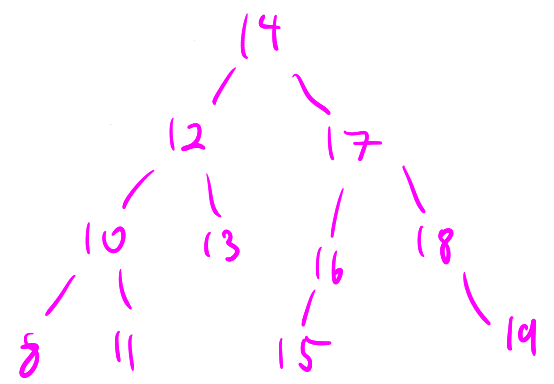
\includegraphics[width=0.3\linewidth]{ex3}
	\end{center}
	Now we are done. The tree is balanced. 	
	
	\end{mdframed}
	
	\subsection{2-4 Trees}
	A 2-4 tree is a\textbf{ non binary search tree} where each node has 2, 3, or 4 children (and therefore 1, 2, or 3 keys) and all \textbf{external nodes have the same depth. }
	
	When we insert, we go down the tree to find where in the key should go. If this causes 5 keys in a node, we split (usually using the third key which gets sent to the parent).
	
	When we delete, we remove the item to delete and replace with inorder successor. If this causes an underflow, we borrow from the parent and fuse the two children together or if the sibling has extra, we take from the sibling, put into the parent, and then steal from the parent. 
	
	\section{Hash Maps}
	We take a problem using a very large table, and use a \textbf{function} to map all data points to a smaller table. 
	
	To resolve collisions, we have a few methods:
	\begin{enumerate}[noitemsep]
		\item Chaining is creating a linked list at each spot in the hash table with items with duplicate hashes.
		\item Linear probing is we will go to the next empty spot linearly (h+0, h+1, h+2, h+3).
		\item Quadratic probing will go to the next spot squared (h+0, h+1, h+4, h+9)
		\item Double Hashing means we have a second hash function that we apply (h(k)+0d(k), h(k)+1d(k), h(k)+2d(k) for $h_j(k)=[h(k)+j^2d(k)]mod N$
	\end{enumerate}

	When we are using any of the methods 2-4, and we delete an item, we cannot just delete the item since we need a record that there was an item there. So we change it to AVAILABLE. This means not to stop searching for a key (since the key could be further along), but we can put a new key there.
	
	\section{Graphs}
	A graph has a set V of all \textbf{vertices}, and a set E of pairs of vertices called \textbf{edges}.
	
	We know that:
	\begin{align*}
		\sum deg(v) = 2m
	\end{align*}
	where m is the number of edges, n is number of vertices, and the degree of vertex v is the number of edges coming out of it. 
	
	A graph is connected if one can get from any vertex to any other vertex along the edges. Basically the graph does not have multiple isolated parts. 
	
	\subsection{DFS}
\textbf{	Depth First Search} is a graph traversial algorithm. 
	
	We start at a random vertex, and then go to the next vertex, then the next one, then the next one, then when we reach the end, we \textbf{backtrack} to visit all the ones we missed. 
	
	We can use a \textbf{stack} to implement this. We go to the first vertex, get all edges, and push to the stack. Then we pop and follow that edge. 
	
	If that edge goes to a new vertex, we then repeat. If it leads to an already visited vertex, we then pop the next edge. Do this until the stack isEmpty.
	
	Its complexity is $O(m+n)$ where the number of edges m can be up to $n^2$ if the graph is an adjacency list. If it is an adjacency matrix, it is always $O(n^2)$.
	
	\subsection{BFS}
\textbf{	Breadth First Search} is a graph traversial algorithm.
	
	We start at a random vertex and then visit \textbf{all adjacent nodes}. Then of all the adjacent nodes visited, we visit all of their adjacent nodes. This creates a \textbf{layer} structure. 
	
	We use a \textbf{queue} to implement this. We go to the first vertex and add all edges to a queue, then we dequeue, go to that vertex, and if not visited, queue all of its edges. Then we dequeue the next edge and repeat. 
	
	Its complexity is the same as DFS.
	
	\subsection{Shortest Path}
	A weighted graph is a graph where all edges have a weight assigned to them. 
	
	\subsection{Dijkstra Algorithm}
	All vertices start with \textbf{distance of infinity}. We start at a vertex A and assign distance 0. 
	
	Then we take all of its incident edges and their weights, and then update all adjacent vertices with their new weights if new weights are better (weight of edge + weight of current verticy).
	
	Now that vertex is in the cloud (done with it). Then we take the smallest weight edge of the entire graph and repeat the previous line. 
	
	We are done once all vertices are in the cloud. 
	
	We use a priority queue for this (min heap).
	
	This is O(mlogn) for a heap, or $O(n^2)$ for an unsorted sequence.  
	
	\subsection{MST}
	
	\subsubsection{PrimJarnik}
	This is almost identical to Dijkstra except rather than keeping track of the whole shotest distance at each vertex, we will just check at vertex V going to K, if VK is shorter than the weight of K. (just weight of edge, do not consider weight of current vertex).
	
	Runs in O(mlogn).
	
	\subsubsection{Kruskal Algorithm}
	With Kruskal, initially each vertex is its own cluster. Then we pick the lowest weight edge and check if each vertex it connects are in different clusters, if so, connect them, if not, move on.
	
	We do this until we run out of edges. 
	
	This works in O((n+m)logn)
	
	\section{Sort}
	These are lots of sorting algorithms:
	
	\begin{tabular}{|c|c|c|c|}
		\hline
		Type & Worst Case & Best Case & Average Case \\
		\hline
		Selection & O(n²) &  O(n²)  &  O(n²)  \\
		\hline
		Insertion &  O(n²)  &  O(n)  &  O(n²)  \\
		\hline
		Bubble &  O(n²)  &  O(n)  &  \\
		\hline
		Heap &  O(nlogn)  &  O(nlogn)  &  O(nlogn)  \\
		\hline
		Merge &  O(nlogn)  &  O(nlogn)  &  O(nlogn)  \\
		\hline
		Quick &  O(n²)  &  &  O(nlogn)  \\
		\hline
	\end{tabular}
	
	\subsection{Mergesort}
	Mergesort is a\textbf{ non in place algorithm} that breaks up the array into 2 parts, each of which gets sorted, and then merges them together. 
	
	This is a recursive algorithm. It gets broken down until there is just 1 element in each side, then it \textbf{merges} those 2 together. 
	
	\subsection{Quicksort}
	Quick sort will choose a \textbf{pivot}, then sort the array by putting all elements \textbf{smaller than the pivot on one side}, and all \textbf{bigger than pivot on the other side}. Then we quicksort each side, finally we put both sides together. 
	
	This can be \textbf{in place}.
	
	\subsection{Bucket Sort}
	Bucket sort puts all items into a \textbf{fixed number of buckets} such as sorting by first letter of the name, there are 26 buckets. 
	
	If there are 2 things that go in the same bucket, we need to ensure to keep the same relative order. This is because Bucket Sort is a \textbf{stable} algorithm. 
	
	If we have n items and N buckets, it takes O(n+N).
	
	\subsection{Radix Sort}
	Radix sort is a bucket sort that can run more than one time. If we are sorting abc, aac, bba, aad, 
	
	We sort once by the first letter to get: abc, aac, aad, bba
	
	Then we sort by the second letter to get: aac, aad, abc, bba
	
	Then by the third letter to get: aac, aad, abc, bba
	
	\subsection{Quadratic Sorts}
	Insertion sort has a sorted part of the array, and then inserts an element from the unsorted part into the sorted part by comparing with each sorted element. 
	
	Selection sort looks for the minimum value then puts into index 0. Then looks for the minimum value from 1-n and puts that into 1, then looks for minimum of 2-n and puts into 2...
	
	Bubble sort goes though the array and swaps while the lower valus is smaller than the higher value. This means each iteration the max goes to the last spot in the array.
	
	
	
	
	
	
	
\end{document}